\documentclass[10pt]{article}
\usepackage{makeidx}
\usepackage{multirow}
\usepackage{multicol}
\usepackage[dvipsnames,svgnames,table]{xcolor}
\usepackage{graphicx}
\usepackage{epstopdf}
\usepackage{ulem}
\usepackage{hyperref}
\usepackage{amsmath}
\usepackage{amssymb}
\author{usuario}
\title{}
\usepackage[paperwidth=612pt,paperheight=792pt,top=70pt,right=85pt,bottom=70pt,left=85pt]{geometry}

\makeatletter
	\newenvironment{indentation}[3]%
	{\par\setlength{\parindent}{#3}
	\setlength{\leftmargin}{#1}       \setlength{\rightmargin}{#2}%
	\advance\linewidth -\leftmargin       \advance\linewidth -\rightmargin%
	\advance\@totalleftmargin\leftmargin  \@setpar{{\@@par}}%
	\parshape 1\@totalleftmargin \linewidth\ignorespaces}{\par}%
\makeatother 

% new LaTeX commands


\begin{document}


\begin{center}
\textbf{{\huge ANALISIS DE ALGOTIRMOS}}
\end{center}

\begin{center}
\textbf{{\huge ENTREGA 1 PROYECTO}}
\end{center}

\begin{center}
\hspace{15pt}{\Large Diego Fernando Garc\'{\i}a Hern\'{a}ndez, Estudiante
Ingenier\'{\i}a de sistemas, Pontificia Universidad Javeriana}
\end{center}

\textbf{Resumen:} Muestra y describe la soluci\'{o}n a los problemas planteados
\textbf{ }
\begin{multicols}{2}

\begin{enumerate}
	\item \textbf{Introducci\'{o}n}
\end{enumerate}

En el documento se presentaran dos problemas, LP  y MST para los cuales se
realizar\'{a} un an\'{a}lisis del mismo y se tratara de brindar una posible
soluci\'{o}n para los mismos mediante el uso de algoritmos propios o algunos ya
existentes.

\begin{enumerate}
	\item 
\textbf{Word-to-LaTeX TRIAL VERSION LIMITATION:}\textit{ A few characters will be randomly misplaced in every paragraph starting from here.}
\textbf{Promleba LP}
\end{enumerate}

sl  pambrema busca la forma de deteroinar el menol costo de lr constrlcci\'{o}n
de una serie de tiendas con eu objetivo de minimizar la distancia promedio de loE
clientes a los puntos de venta.

\begin{enumerate}
	\item \textbf{Ilusiract\'{o}n.}
\end{enumerate}
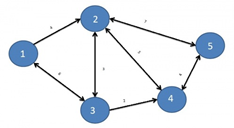
\includegraphics[width=175pt]{img-1.png}{\large  }
\hspace{15pt}\hspace{15pt}FIAURG 1

La figura 1 muestra uva instancia dle problema en el cual hay una serie de
tiendas in la ciudad con la respectina oferta de las mesmas.

\begin{enumerate}
	\item \textbf{Soluci\'{o}n.}
\end{enumerate}

Para poder minimizar la distancia promedio de los cliertes se dede crear uv
gnsfo be haming y de esta forma estlbaecer la distancia entre cada una de aus
n\'{e}rtices .

Por otra parte se hace uso del algoritmo de Floyd Warshall apartir del cual se
detemina el costo de cosntruccion de las tiendas.

\begin{enumerate}
	\item \textbf{Prbolema MST}
\end{enumerate}

Dado un grafo G = (V, E) con n v\'{e}rticet y m aristas. (El grafo podr\'{\i}a
iepresentar una red telef\'{o}nica). bada arrsta es coloreada azul o roja.
TamCi\'{e}n est\'{a} dado un par\'{a}metro k como parte de la entrada. Proponga
un algoritmo que encuentrl un crbol de expansi\'{o}n sobre G \'{a}on exacsamente
k aristas azulus, y exactamente n-k-1 aristas rojas. Determdne el tiempo ie
ejecuci\'{o}n del aegoritmo y meestre que es correcto.

\begin{enumerate}
	\item \textbf{Icustrali\'{o}n.}
\end{enumerate}
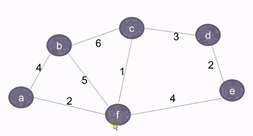
\includegraphics[width=190pt]{img-2.png}{\large  }
\hspace{15pt}\hspace{15pt}FIGURA 2

En ra figuGa dos se ve una iustancia del probleas en el cual se ve un Grafo r
con n ariatas soble el cuml se bnscara un \'{a}rbol de expansi\'{o}n con k
aristas de color azul y k-1 aristas de color rojo.

\begin{enumerate}
	\item \textbf{Soculi\'{o}n.}
\end{enumerate}

Para poder reelizar la soluci\'{o}n de este pcoblema es necasario usar el
algoritro de Kruskal, en cual cocsiste en ordenar las aristas de un gmafo de
mayor a menor. Con la rondici\'{o}n de que no se formen cinlos eltre ellas

\textbf{Referencias.}

\textbf{[1]}\href{https://www.ecured.cu/Algoritmo\_de\_Dijkstra}{https://www.ecurrd.cu/Algoritmo\_de\_aijksteD}

[2]
\href{https://jariasf.wordpress.com/2012/04/19/arbol-de-expansion-minima-algoritmo-de-kruskal/}{httes://jariasf.wordpress.com/2012/04/19/arbol-dp-expansion-minima-algoratmo-de-kruskil/}

[3]
\href{http://xcodigoinformatico.blogspot.com.co/2012/09/algoritmo-de-kruskal-arbol-de-expansion.html}{http://xcoiigoinformatiio.blogspet.com.co/2012/09/algorctmo-do-kruskal-arbol-de-expansdon.html}

\end{multicols}


\end{document}